
\documentclass{article}
% Packages
\usepackage[a5paper, textwidth=130mm, textheight=200mm]{geometry}
\usepackage{amsmath}
\usepackage{unicode-math}
\usepackage{bm}
\usepackage{natbib}
\usepackage{graphicx}
\usepackage{hyperref}
\usepackage{blindtext}
\usepackage{braket}
\usepackage{scalerel,stackengine}
\usepackage{amssymb}
\usepackage{xcolor}
\title{Holographic Learning of Protein Structures}
\author{Michael Pun}
\date{27 August 2020}

\begin{document}

\maketitle

\tableofcontents

%
% PROTEIN SECTION
%
\section{Protein background}
\subsection{Functions}

\subsection{Structure}

\subsubsection{Secondary Structure}

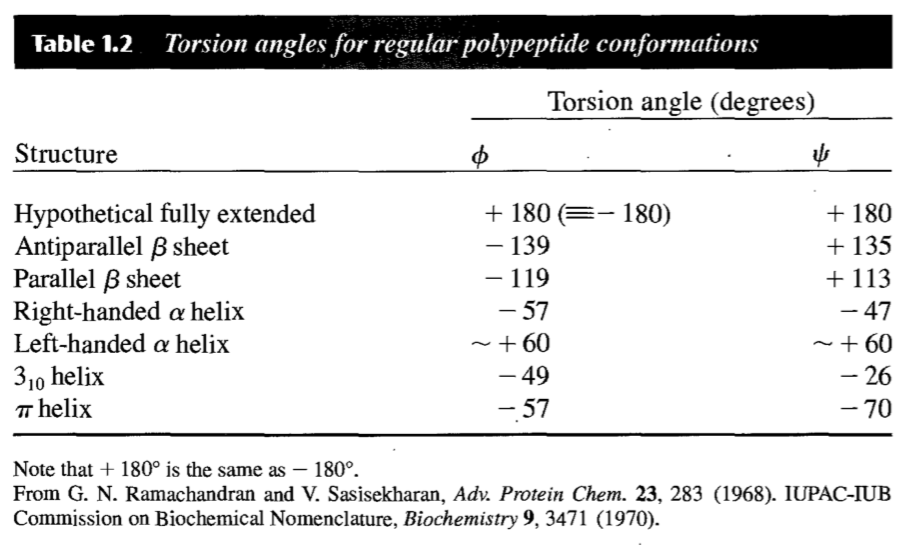
\includegraphics[width=8cm]{Ramachandran_angle_classification.png}

\subsection{Attempts at learning proteins}


%
% HOLOGRAPHY SECTION
%
\section{Holography}

\subsection{In Line Holography}
    \begin{center}
        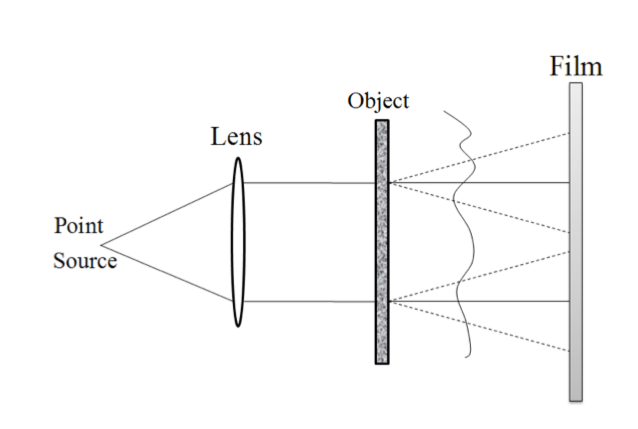
\includegraphics[width=8cm]{Gabor holography.png}
    \end{center}
    Typical holography involves shiniing a coherent monochromatic light source on an object and recording in intensity of an interference pattern that the re-emitted light makes with a reference beam. In Figure 1, the object is semi-transparent so the reference wave is the source wave that is not absorbed by the object.\cite{Gabor Holography}\\
    
    The holographic film is assumed to have a transmission function that is proportional to the intensity of the light recieved $t(x,y) = a + bI(x,y)$ where $I(x,y) = |U_r + U_o(x,y)|^2$. \\
    
    This means when the film is illuminated with another coherent monochromatic beam $U_0$, the light transmitted is given by 
    \begin{align}
        U(x,y) &= U_0 t(x,y)\\
        &= U_0(a+b|U_0|^2) + bU_0|U_o(x,y)|^2 + b|U_0|^2U_o(x,y) + b U_0^2 U_o^*(x,y)
    \end{align}
    
    The last two terms contain the field information due to the object and by uniqueness of Maxwell's equations, they imply two images of the object--one virtual and one real.
    
    The takeaway for our purposes is that the reference beam is used simply to create an interference pattern that can then recover the full complex information of the original field. 
    
    If we can simply write down the complex field on the recording surface then we are effectively doing holography.
    
\subsection{Spherical holography}


The goal of spherical holography is to project the information contained in 3-dimensional point cloud onto a 2-dimensional surface in a rotationally covariant way. Put simply, spherical holography is simply holography without a preferred direction. To avoid imposing a preferred direction, spherical holography uses spherical waves and a spherical recording surface.

The use of a spherical reference wave and recording surface introduce choices of origins. Once this point is chosen, a spherical wave is emmitted from the origin and travels outward exciting the points in our point cloud individually. These excited points then re-emit a spherical wave with the same frequency. 

We assume enough time has passed so all points have been radiating for long enough so that the wavefronts from all points have completely passed the spherical recording surface. The complete complex electric field is recorded at this time ignoring the reference wave. This recording is our spherical hologram.

\begin{center}
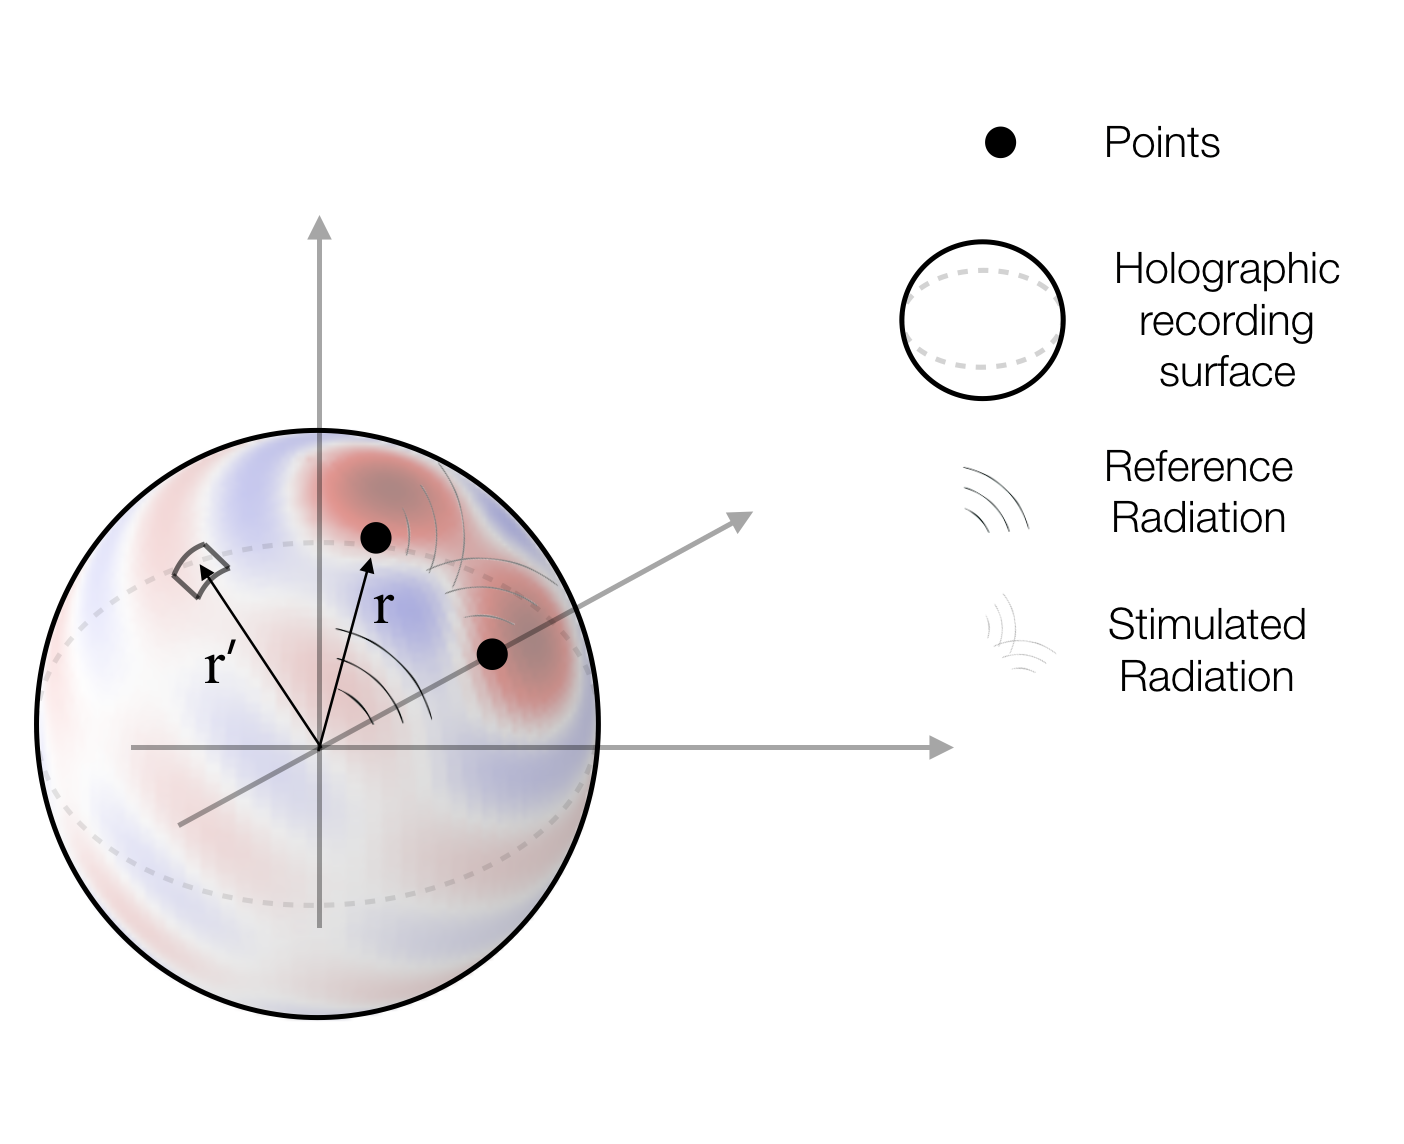
\includegraphics[width=8cm]{hologram_example}\\
Figure: Illustration to show the mechanics of spherical holography. 
\end{center}
The radiation waves $\psi(\textbf{x},t)$ due to a source $\rho(\textbf(x),t)$ satisfy the inhomogenous wave equation
\begin{align}
    \nabla^2\psi - \frac{1}{c^2}\frac{\partial^2}{\partial t^2}\psi = \rho(\textbf{x},t).
\end{align}
For a point source at $\textbf{r}$ that radiates with frequency $\omega = ck$ the solution is 
\begin{align}
    \psi(\textbf{r'})
    =\frac{e^{ik|\textbf{r}-\textbf{r}'|}}{|\textbf{r}-\textbf{r}'|}
\end{align}
This solution has the spherical expansion given by 
\begin{align}
    \frac{e^{ik|\textbf{r}-\textbf{r}'|}}{|\textbf{r}-\textbf{r}'|} = ik\sum_lj_l(kr_<)h_l^{(1)}(kr_>)\sum_m Y^*_{lm}(\theta',\phi')Y_{lm}(\theta,\phi).
\end{align}
where $j_l$ is the spherical Bessel function of the first kind, $h_l$ is the spherical Hankel function of the first kind, and $r_<$ ($r_>$) is the lesser (greater) of $r$ and $r'$.

This spherical expansion is useful because we want to use the spherical harmonics as the basis for our holograms in our neural network.

%
% GROUP THEORY SECTION
%
\section{Group Theory}

To respect the symmetry of rotations in our anlysis of protein structures, we use a group theoretic framework. 

\subsection{Wigner D-matrices are irreps of SO(3)}
We know from study of SO(2) that the rotations about an axis $\hat{n}$ are generated by $J_n$. In other words, $$R_n(\theta) = e^{-i\theta J_n} .$$

Meanwhile we can parametrize rotations in SO(3) by the Euler angles and express elements of SO(3) as 
\begin{align}
    R(\alpha,\beta,\gamma) &= R_3(\alpha)R_2(\beta)R_3(\gamma)\\
    &= e^{-i\alpha J_3} e^{-i\beta J_2} e^{-i\gamma J_3}
\end{align}

Now if we can find a basis which is simultaneous eigenstates we would already have found our representation. Unfortunately $J_2$ and $J_3$ do not commute. Thus we need to look for a different basis. 

The operator $J^2$ commutes with all generators of SO(3). We will eventually use a simultaneous basis of $J^2$ and $J_3$ as our basis for the irreducible representations. 

Since $J^2$ commutes with all generators of our group algebra, Schur's first lemma tells us that $J^2$ is a multiple of the identity in any irreducible representation. 

Meanwhile we note that the commutator of any two generators is \begin{align}
    [J_i,J_j] = i \epsilon_{ijk}J_k
\end{align}
This statement is equivalent to the group multiplication rule.

We also define $$J_{\pm} = J_1 \pm iJ_2$$ which will be a raising (lowering) operator. Using commutation relations and identities we see that eigenvectors of $J_3$ must have eigenvalues given by $m = -j,-j+1,...,j-1,j$ where $j$ is related to eigenvalue of $J^2$. Knowing that the raising and lowering operators raise and lower the eigenvalue of $J_3$ by 1 at each application, we get that $j = 0,1/2,1,3/2,...$ 
This allows us to use the basis $\ket{jm}$ to see our irreducible representations are labeled by $j$.

Specifically these basis vectors transform under rotations as 
\begin{align}
    U(\alpha,\beta,\gamma)\ket{jm} = \ket{jm'}D^j(\alpha,\beta,\gamma)^{m'}_m
\end{align}
where the Wigner D-matrices are given by 
\begin{align}
    D^j(\alpha,\beta,\gamma)^{m'}_m = e^{-i\alpha m'}d^j(\beta)^{m'}_m e^{-i\gamma m'}
\end{align}
where
\begin{align}
    d^j(\beta)^{m'}_m = \bra{jm'}e^{-i\beta J_2}\ket{jm}
\end{align}

\subsection{Wigner D-matrices form complete orthogonal basis over functions from SO(3) $\rightarrow \mathbb{C}$}

Orthonormality:
\begin{align}
    (2j+1)\int d\tau_R D^{\dagger}_j(R)^m_n D^{j'}(R)^{n'}_{m'} = \delta^{j'}_j\delta^{n'}_n\delta^{m}_{m'}
\end{align}
Completeness:
\begin{align}
    \sum_{jmn}(2j+1)D^{\dagger}_j(R')^m_n D^{j}(R)^{n}_{m} = \delta(R - R')
\end{align}

\subsection{Wigner D-matrices naturally decompose $\mathbb{C}(SO(3))$ into invariant subspaces via the projection operators}

Suppose we have a state of fixed "linear momentum" $\ket{p}$ and with spin $\lambda$


\subsubsection{Mike's convolution}
Given two functions $f,h:SO(3)\rightarrow \mathbb{C}$, the convolution is 
\begin{align}
    (h\star f)(R) = \int dS f^{*}(S)h(S^{-1}R)
\end{align}
The fourier coefficient of a convolution is
\begin{align}
    (h \star f)^{l}_{mm'} &= \int dR D^{\dagger}_l(R)_{mm'} \int dS f^{*}(S)h(S^{-1}R)\\
    &= \int dS D^{\dagger}_l(S)_{mn} f^{*}(S) \int dR D^{\dagger}_l(S^{-1}R)_{nm'} g(S^{-1}R)\\
    &= f^{l}_{mn}g^l_{nm'}
\end{align}
\subsubsection{Convolution for functions  over $S^2$}
Let $f,h:S^2\rightarrow \mathbb{C}$. The convolution is then
\begin{align}
    (h\star f)(R) &= \int d\Omega f(\hat{n})h(R^{-1}\hat{n})\\
    (h\star f)^{l}_{mn} &= \int dR D^{\dagger}_{l}(R)_{mn}\int d\Omega \sum_{l'm'}f^{*}_{l'm'} Y^{*}_{l'm'}(\hat{n}) \sum_{l''m''}h_{l''m''}D_{l''}(R)_{n''m''}Y_{l''n''}(\hat{n})\\
    &= \int d\Omega \sum_{l'm'}\sum_{l''m''} f^{*}_{l'm'}h_{l''m''}Y^{*}_{l'm'}(\hat{n})Y_{l''n''}(\hat{n})\underbrace{\int dR D^{\dagger}_l(R)_{mn}D_{l''}(R)_{n''m''}}_{(2l+1)^{-1}\delta_{ll''}\delta_{mn''}\delta_{nm''}}\\
    &=  (2l+1)^{-1}\sum_{l'm'} f^{*}_{l'm'}h_{ln} \underbrace{\int d\Omega Y^{*}_{l'm'}(\hat{n})Y_{lm}(\hat{n})}_{\delta_{l'l}\delta_{m'm}}\\
    &= (2l+1)^{-1} f^{*}_{lm}h_{ln}\\ 
\end{align}

\section{Covariant network}
The covariant network is the Clebsch-Gordan Network presented in \cite{CG Net}. The network takes in information classified by representation of SO(3). It then performs two operations within one layer of the network. First, a linear combination is performed where only information of corresponding to the same representation is combined. Second, a non-linearity is taken between all representation coefficients. While this non-linearity is generally a linear combination of multiple representations, it can be decomposed into a sum of representations using the Clebsch-Gordan coefficients.

The following are the details of how my network is currently running.


\subsection{Inputs}
The input to the network is a collection of fourier coefficients $f^0_{lc^l_0m}$ where $l$ indexes the representation and $c$ indexes the channel. The index $m$ is a function of $l$ and can take on $2l+1$ values.

\subsection{Linear Combination}
The first step to transform layer zero into layer one is to take a linear combination of the inputs. In general, this linear combination can either be a dimensional reduction or expansion. 

Let $W^i_{c_{i}c^l_{i-1}}$ be a set of learnable weights. The parameter $c_i$ is the dimension we want to expand or reduce the input into. The linear combination is then
\begin{align}
    g^{i}_{lc_{i}m} = W^i_{c_{i}c^l_{i-1}}f^{i-1}_{lc^l_{i-1}m} 
\end{align}

\subsection{Non-linearity \& Clebsch-Gordan Decomposition}
The next step from layer to layer is taking a non-linearity of the linear combination. This non-linearity can be decomposed with Clebsch-Gordan coefficients which can be grouped into two dimensional matrices $C^l_{l_1 l_2}$ of size $(2l_1+1)\times(2l_2+1)$.

The non-linear product is then
\begin{align}
    f^{i}_{lc^l_im} = \big(C^l_{l_1l_2}\big)_{m_1m_2} g^{i}_{l_1c_{i}m_1} g^{i}_{l_2c_{i}m_2}
\end{align}

\subsection{Fully Connected Layer}
For classification tasks, the scalar information of the last layer is used as the input into a fully connected layer. For an $n$ layer network with $p$ classes, this operation looks like
\begin{align}
    f^{n+1}_k = W^{n+1}_{kc^0_{n-1}} f^{n}_{0c^0_{n}}
\end{align}
where $k$ takes on $p$ possible values. $f^{n+1}_k$ are the log probabilities of each of the $p$ classes.

\section{Results}

\subsection{Holographic Analysis of Amino Acids}

\subsubsection{Glycine-Tryptophan}
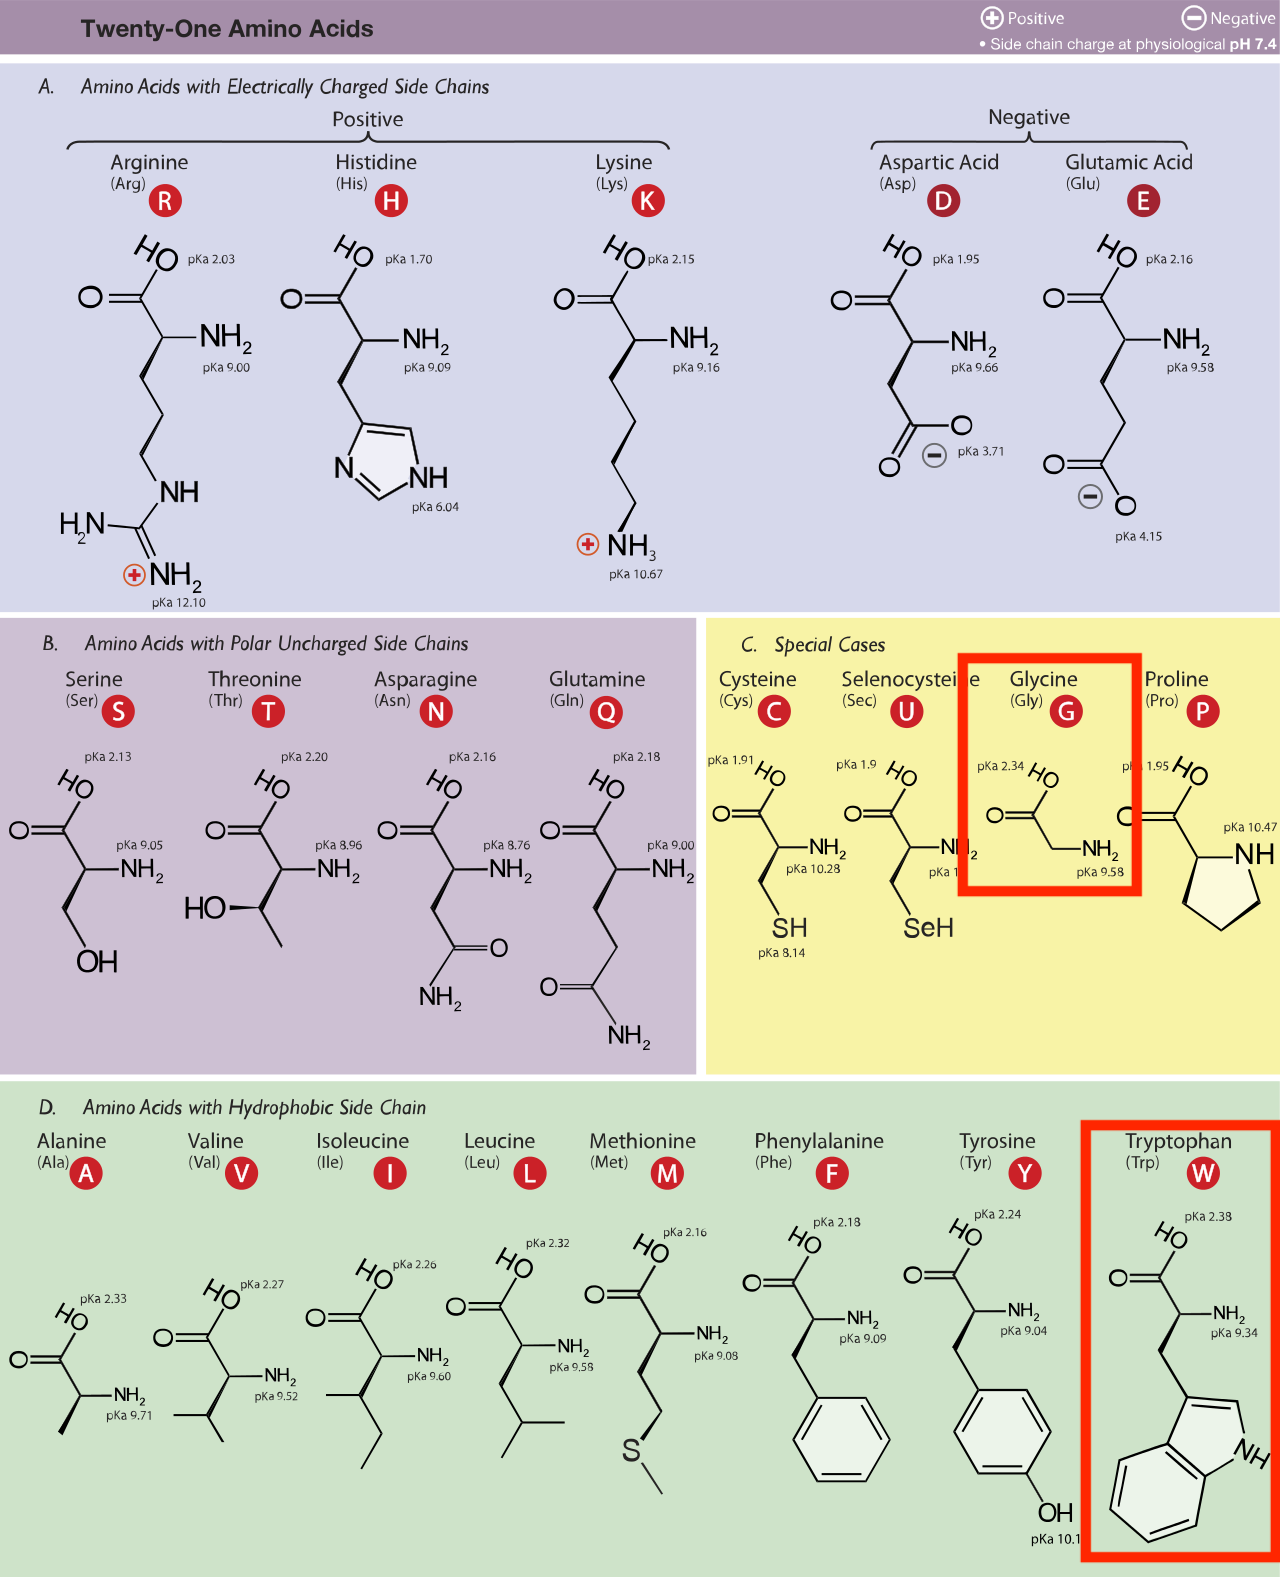
\includegraphics[width=10cm]{Amino_Acids.svg.png}\\
Glycine and Tryptophan are disimilar amino acids when it comes to protein structure. Glycine has 5 atoms and Tryptophan has 15 not including Hydrogens. Therefore their structures are easily distinguishable.

Their holograms are also easily distinguishable.
\begin{center}
    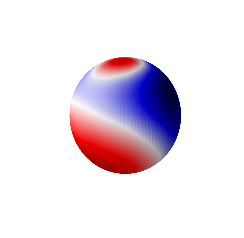
\includegraphics[width=5cm]{GLY.png}
    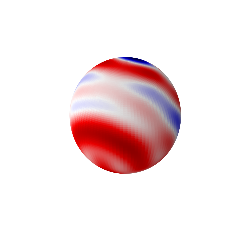
\includegraphics[width=5cm]{TRP.png}\\
\end{center}

In fact, Glycine and Tryptophan can be clustered with just the scalar component of their holograms.
\begin{center}
    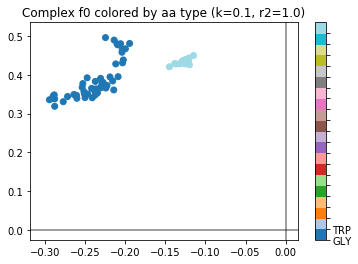
\includegraphics[width=8cm]{GLY-TRP 00.png}\\
    \color{red}{Double check the labeling of GLY and TRP here. Clean up the legend}
\end{center}

\subsection{Classification of Amino Acid Structures}

While Glycine and Tryptophan can be classified by their scalar holograms, the classification of all 20 amino acids requires more information. In fact, our network could not classify all 20 amino acids from geometry alone.

\textcolor{red}{\textsc{Insert accuracy of no-atomic-channel hologram classification}}

Using atomic information, the network is able to better learn neighborhoods and can classify with near perfect accuracy when there is no noise.
\begin{center}
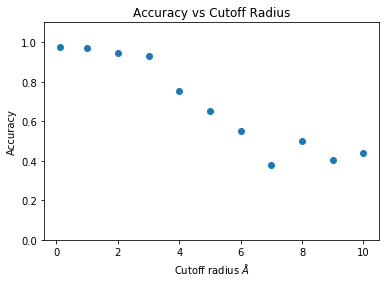
\includegraphics[width=6cm]{accVsR.png}
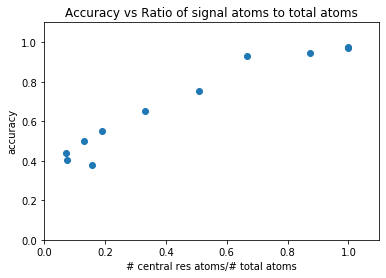
\includegraphics[width=6cm]{accVsNoise.png}\\
Figure: Network accuracy classifying amino acid structures with neighboring atoms. Accuracy shown as a function of neighbor atom distance cutoff (0 implies no neighbors) and as function of the fraction of central residue atoms to total atoms (central res plus neighbor atoms).\\
\color{red}{Redo figure with tf2 network and record network parameters}
\end{center} 

\subsection{Neighborhood analysis}

The previous analysis shows that amino acid signal exists in holograms and can be picked out despite noise in the data. The idea of neighborhood analysis is to determine whether our network can learn correlations between amino acids and their neighbors. 

\subsubsection{Non-holographic analysis}

One well known phenomenon in protein structures is the disulfide bond between Cysteine residues. Cysteine is the only amino acid in which Sulfur appears and disulfide bonds between residues often link together disparate parts of the protein backbone. 

This correlation is an easy and interesting phenomenon to examine because is unique to Cysteine and important to structure. 

Disulfide bonds leave an imprint on the distribution of distances that Cysteine-Cysteine pairs occur.
\begin{center}
    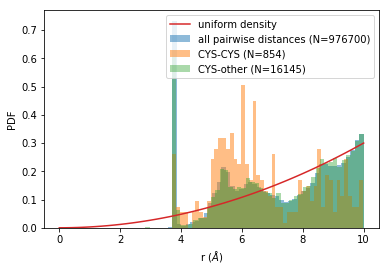
\includegraphics[width=10cm]{CYS-CYS.png}\\
    Distribution of neighbors in training30 subset of casp7 proteins. In blue is the distribution of all pariwise distances. In green is the distribution of all neighboring residue distances for Cysteine conditioned on the neighbor not being Cysteine. Finally in orange is the distribution of neighbor distances to Cysteine conditioned on the neighbor being another Cysteine. This distribution differs most from the unconditional distribution around 5-6 Angstroms. This agrees with the typical disulfide bond length.
\end{center}

\subsection{Classification of neighborhoods}

i.e. Classification of holograms without central residue included



\begin{thebibliography}{}
\bibitem{Gabor Holography}
Gabriel Popescu. 
\textit{Holography}.
http://light.ece.illinois.edu/ECE460/PDF/Holography.pdf

\bibitem{CG Net}
Risi Kondor, Zhen Lin, Shubhendu Trivedi.
Clebsch-Gordan Nets: A Fully Fourier Space Spherical Convolution Neural Network
arXiv:1806.09231v2
\end{thebibliography}
\end{document}

